% !TEX root = ../gnss_interference_resistant_thesis.tex
\documentclass[main.tex]{subfiles}

\begin{document}

\subsection{KerberosSDR fazinės sinchronizacijos matavimas}

Fazinei sinchronizacijai tarp imtuvų matuoti naudojamas integruotas triukšmo generatorius,
tačiau šį kartą naudosime kitą metodą fazės skirtumo gavimui.

Fazės skaičiavimui pasinaudosime jau turimu koreliacijos rezultatu. Kadangi koreliacija
atliekama su kompleksiniais skaičiais, tai koreliacijos rezultatas irgi gaunamas kompleksinis.
Absoliuti koreliacijos vertė parodo koreliacijos koeficientą, o kompleksinio skaičiaus kampas
parodo signalų fazės skirtumą.

\begin{figure}[h]
    \begin{centering}
    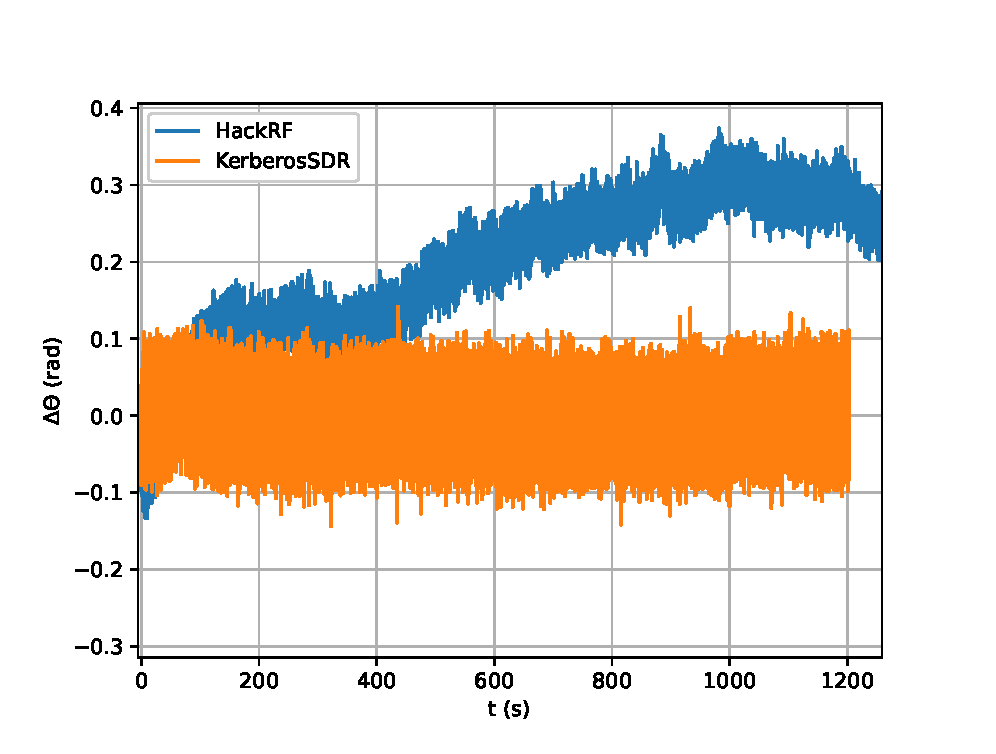
\includegraphics[scale=1.0]{drawings/hackrdf_vs_kerberos_phase_over_time.eps}
    \par\end{centering}
    \protect\caption{\label{fig:phase_stability}Fazės stabilumas HackRF ir KerberosSDR imtuvų.}
\end{figure}

\ref{fig:phase_stability}~pav. aiškiai matome, kad KerberosSDR imtuvo fazė yra 
stabilesne už HackRF. KerberosSDR vidutinis fazės nuokrypis per 20 minučių nekito,
o HackRF imtuvo fazė pasikeitė per $0,35\ \mathrm{rad}$. Toks fazės nuokrypis, pagal
\refeq{eq:phase_shift_antenna_angle} lygtį, reikštų apie $6\degree$ spindulio maksimumo nuokrypį.
Kadangi spindulio formavimas bus vykdomas tik su keturiomis antenomis ir tokiu atveju
spindulio plotis yra daug didesnis, tai nėra reikšmingas fazinis nuokrypis.

Taip pat kaip ir HackRF atveju, kiekvieną karta įjungus imtuvus, pradinis fazių skirtumas
tarp imtuvų yra atsitiktinis, todėl prieš kiekvieną matavimą reikia atlikti imtuvo kalibravimą.
KerberosSDR atveju atlikti kalibravimą yra lengviau, dėl integruoto triukšmų generatoriaus.

\end{document}
